\documentclass[a4paper, 10pt]{report} % perhaps book?
\usepackage{graphicx}
\usepackage{url}
\begin{document}
\title{Mufasa Handbook}
\author{Merlijn Wajer}
\maketitle

\chapter{Introduction}

\emph{This is the official Mufasa Documentation.
The main purpose of this document is to provide a clear view on Mufasa's 
interal structure. This guide is aimed at developers and other persons
interested in project Mufasa.}

\section{What is Mufasa?}

Mufasa is a project that aims to create the Mufasa Macro Library (MML).
As a side project, the project also tries to create a simple but effective
user interface to the Mufasa Macro Library. This is achieved with the
Pascal interpreter PascalScript\footnote{\url{http://www.remobjects.com/ps.aspx}}
combined with a wrapper for the MML.

Mufasa is:
\begin{itemize}
	\item Object Oriented. Since OOP also increases the abstraction of
		  certain tasks/parts, the code is much easier to maintain and
		  comprehend.
	\item Free Software, as in, Free.\footnote{License here}
	\item Cross platform. Currently the supported platforms are Linux 
		  (32 and 64 bit) and Windows (32 and 64 bit).
		  Mac support is planned; but currently halted due to lack of a
		  Mac computer.\footnote{Virtual Machines are an option;
		  but currently Darwin is not supported on Virtualbox.}
	\item A community project; the SRL community\footnote{
			\url{http://www.villavu.com}}
		  is widely known for it's maturity and open-mindedness.
	\item Mufasa is actively maintained. It also has a bugtracker,
		  a wiki, and a forum.
\end{itemize}

\pagebreak

\subsection{Mufasa Macro Library}

The MML's main features are:
\begin{itemize}
	\item Mouse control.
	\item Keyboard control.
	\item Screen capturing and analyzing.
	\item Providing several methods to analyzing the screen; among these
		  are DTM's and Bitmaps.
	\item API's to open files and web pages.
\end{itemize}

\subsection{Mufasa GUI}

As mentioned in the introduction, the Mufasa GUI uses Pascal Script as 
interpreter. \\ 

A non-OOP MML wrapper has been created only for the purpose
of exporting MML functionality to Pascal Script. 
This allows the user to use MML functions in their so called `Scripts'. \\
A more detailed specification will be given once we have explored the MML.

\chapter{The Mufasa Macro Library and it's Core Classes}

The Mufasa Library consists out of one class that combines all the other
classes, the \textbf{Client} class.

\section{The Client Class}

The \textbf{Client} class is the main Class, and is designed 
to run seperately from the User Interface.
The Client class is mainly designed to be a container for other classes.
If one wants to use the MML as a whole, he will only need the use 
the Client class.

\begin{figure}[ht]
	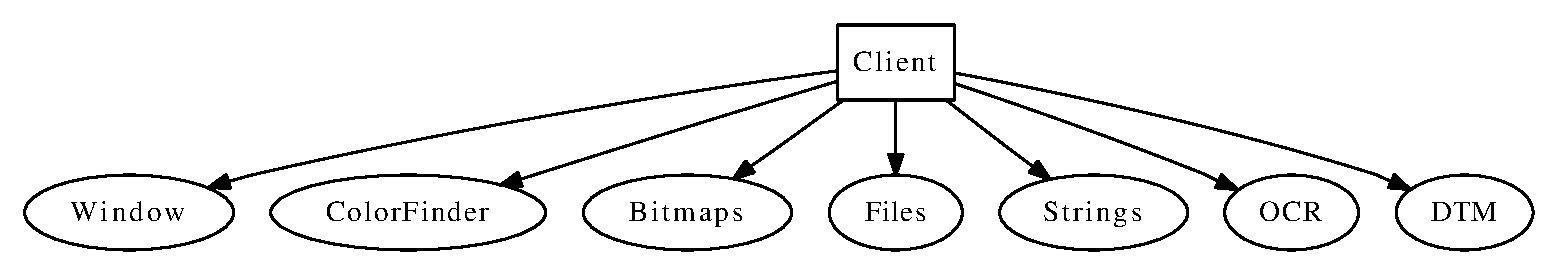
\includegraphics[scale=0.4]{Pics/Client_Classes}
	\caption{Classes that the Client contains.}
\end{figure}

\pagebreak

\section{The Window Class}

The \textbf{Window} class manages the core functionality for retreiving Window data,
such as the actual pixel data and the position and dimension of a window. \\

The Window class' main purpose is to form a cross platform class to retrieve
window information; no other class than the Window class should have to do
any platform-specific function calls to retreive window data; this is all
abstracted by the Window class.\footnote{This implements the so-called 
encapsulation of functionality.} \\

The Window class:

\begin{figure}[ht]
	\includegraphics[scale=0.4]{Pics/Window}
	\caption{Simplified structure of the Window class}
\end{figure}

Figure 2.2 is ofcourse a highly simplified representation of the Window class;
the real class implements several other features. Among those are copying
(parts) of a window to a bitmap, methods to set a window as target, and
a feature that allows the user to ``Lock'' the Windows' current data in
Mufasa-maintained memory. \\

Quick overview of functions:

\begin{itemize}
	\item ReturnData
	\item FreeReturnedData
	\item GetDimensions
	\item SetTargetWindow
	\item SetTargetIntArray
	\item SetTargetXWindow
	\item GetPixel
\end{itemize}

Together, these functions form the core of the window management.
However; to fake user input, a programmer also needs the ability to 
manipulate user input. Which brings us to the next MML Core class.

\section{The Input Class}

The \textbf{Input} Class is the class that takes care of all the input. \\
As one can see in Figure 4, MML aims to support both Silent and non Silent 
Input. Since the Input heavily differs per operating system, 
the Input class should have a general way of sending keys,
possibly at the expense of losing some functionality.

\subsection{Silent Input}

So what is Silent Input?
We\footnote{The Designers and Developers of Mufasa} define Silent Input as
methods to manipulate the user's mouse and keyboard, without visually using
them. So what does this mean? \\

This basically means that you will still be able to use your mouse while
MML is performing mouse operations on your targetted window/client.

However, silent input is very hard to implement, and often hardly supported
by host operating systems. Often silent mouse or keyboard input is simply 
ignored. So in general is it advised to stick to non silent input.


\begin{figure}[ht]
	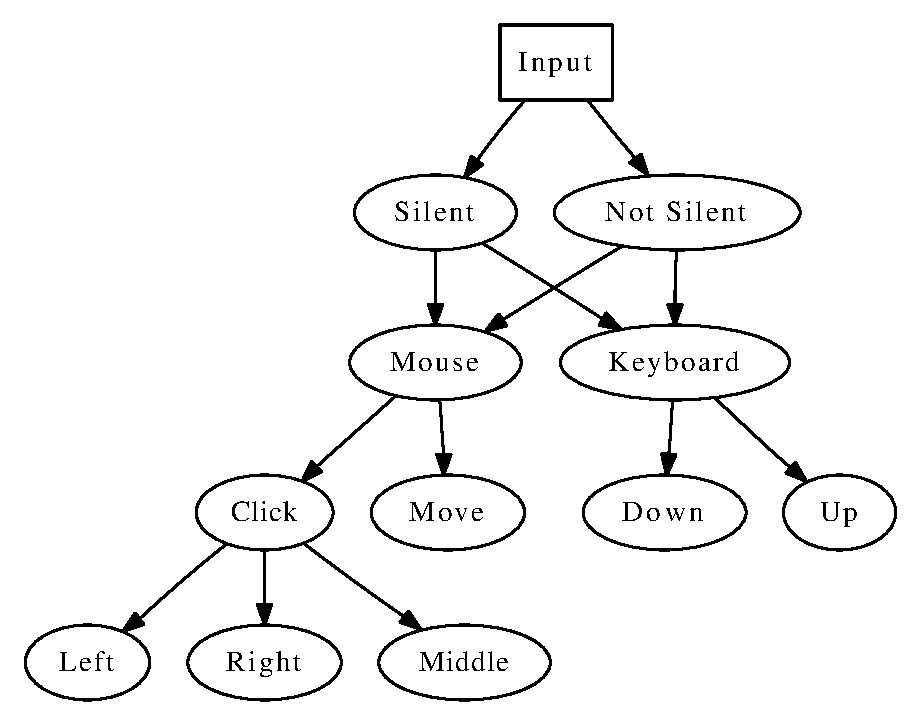
\includegraphics[scale=0.4]{Pics/Input_Diag}
	\caption{Input Functionality.}
\end{figure}
\section{The Colour Convertions Include}

The \textbf{Colour Conversions} unit contains pascal code to quickly convert
one colour type to another. It also adds support for comparing colours.
The reason this is not a class, is because constantly dereferencing a class
to call a single\footnote{Small} function won't do the speed of a program any 
good. There also wasn't really a need for a class,
since none of these functions need to be initialized in any way.

\section{The Colour Class}

The colour class is a Class that does all the colour identfying and locating
work. (A function like FindColor does this)
The colour class uses the Colour Convertions unit for several of it's
functions.

A FindColor-derivative function in Mufasa exists generally out of the following
steps:
\begin{itemize}
	\item Retrieve Client Data.
	\item Loop over the data, possibly with a special (spiral) algorithm.
	\item Check the current pixel data against another colour, possibly 
		  with tolerance.
	\item Free the Client Data.
	\item Return found point(s).
\end{itemize}

\begin{figure}[ht]
    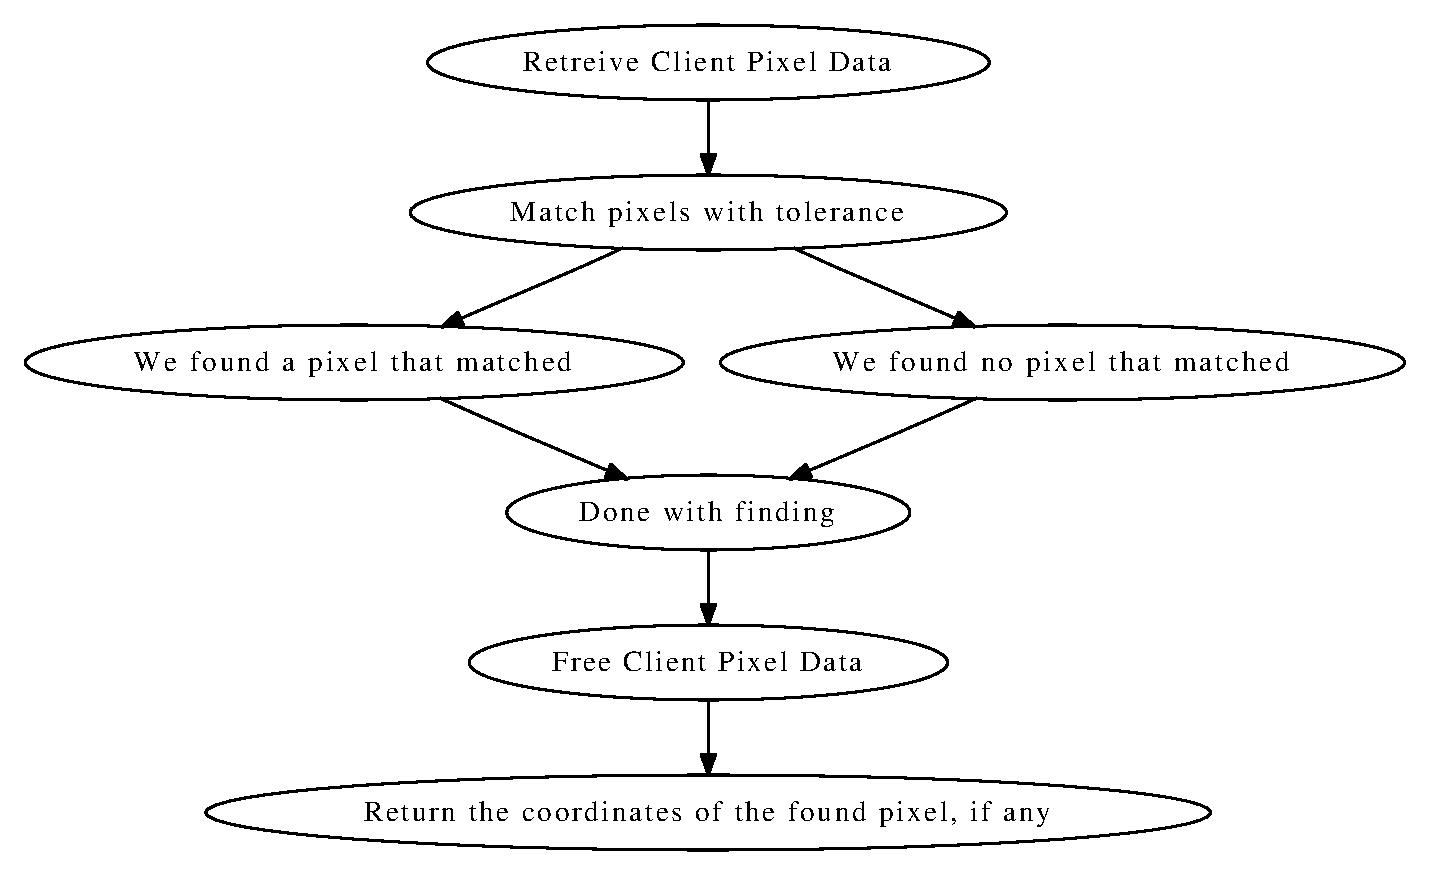
\includegraphics[scale=0.4]{Pics/FindColor}
    \caption{A basic find colour.}
\end{figure}

\chapter{DISREGARD ANYTHING PAST THIS}

\section{DTMs and the DTM Class}


\section{Bitmaps and the Bitmaps Class}



\section{Notes on the previously mentioned classes}


\section{More On The Core Classes}

The previously mentioned MML classes are considered to be the absolute core of the library. (Although one could argue that even the Colour class isn't part of the core classes.)

With these classes most functions that Mufasa will contain can be created. if you can make FindColor, you can make FindColorsSpiralTolerance, they don't really differ a lot. The same goes for DTM's, OCR and Bitmaps. Mouse and keyboard functions will be done with the Input class.

The MML contains more classes, and they will mainly utilize the previous mentioned classes.
It is essential to understand the Classes architecture to fully understand Mufasa.
Before work on other classes will be done, the core classes must be finished and stable.

A good rule of thumb is the following: any units that make extensive use of Compiler Directives, are considered a core unit.

\end{document}
